\chapter{El agua en todos sus estados}\label{ch:g6:water-states}

Llevas persiguiendo al agua por sus estados desde tu segundo año de
colegio: hielo, agua, vapor; muñecos de nieve que se funden y
ventanas empañadas. Este año la persecución se convierte en
contabilidad. Cuando el hielo \omterm{def:g2:ice-water-steam:meltfreeze}{se derrite}, ¿se pierde algo de
sustancia? Cuando el agua \omterm{def:g2:ice-water-steam:meltfreeze}{se congela}, ¿por qué revientan las
tuberías? Con \omterm{def:g3:levers-and-scales:scale}{balanzas} y probetas en la mano, auditamos los tres
estados del agua.

\section{Los tres estados, con sus etiquetas formales}

\begin{definition}[Los seis cambios de estado]\label{def:g6:water-states:changes}
Entre sus tres estados, el agua tiene seis puertas, cada una con su
nombre científico:
\begin{enumerate}
  \item \omterm{def:g3:solids-liquids-gases:solid}{sólido} $\to$ \omterm{def:g3:solids-liquids-gases:liquid}{líquido}: \emph{fusión}\index{fusión};
        \omterm{def:g3:solids-liquids-gases:liquid}{líquido} $\to$ \omterm{def:g3:solids-liquids-gases:solid}{sólido}:
        \emph{solidificación}\index{solidificación} (la congelación);
  \item \omterm{def:g3:solids-liquids-gases:liquid}{líquido} $\to$ \omterm{def:g3:solids-liquids-gases:gas}{gas}:
        \emph{vaporización}\index{vaporización} --- ruidosa y rápida
        en la ebullición, silenciosa y fresca como evaporación;
        \omterm{def:g3:solids-liquids-gases:gas}{gas} $\to$ \omterm{def:g3:solids-liquids-gases:liquid}{líquido}:
        \emph{condensación}\index{condensación};
  \item \omterm{def:g3:solids-liquids-gases:solid}{sólido} $\to$ \omterm{def:g3:solids-liquids-gases:gas}{gas} directamente:
        \emph{sublimación}\index{sublimación}, y \omterm{def:g3:solids-liquids-gases:gas}{gas} $\to$
        \omterm{def:g3:solids-liquids-gases:solid}{sólido} directamente --- puertas más raras, pero reales: las
        plumas de escarcha de una ventana helada crecen directamente
        del vapor invisible y se saltan por completo el \omterm{def:g3:solids-liquids-gases:liquid}{líquido}.
\end{enumerate}
\end{definition}

\begin{omfigure}
\begin{tikzpicture}[scale=0.85]
  \node[draw, thick, omDef, font=\small, minimum width=1.9cm,
    minimum height=0.85cm] (ice) at (1.2,0) {hielo};
  \node[draw, thick, omDef, font=\small, minimum width=1.9cm,
    minimum height=0.85cm] (wat) at (5.7,0) {agua};
  \node[draw, thick, omDef, font=\small, minimum width=1.9cm,
    minimum height=0.85cm] (vap) at (10.2,0) {vapor};
  \draw[-Stealth, very thick, omThm] (2.25,0.28) -- (4.65,0.28);
  \node[above, font=\footnotesize, omThm] at (3.45,0.42) {fusión};
  \draw[-Stealth, very thick, omDef] (4.65,-0.28) -- (2.25,-0.28);
  \node[below, font=\footnotesize, omDef] at (3.45,-0.42)
    {solidificación};
  \draw[-Stealth, very thick, omThm] (6.75,0.28) -- (9.15,0.28);
  \node[above, font=\footnotesize, omThm] at (7.95,0.42)
    {vaporización};
  \draw[-Stealth, very thick, omDef] (9.15,-0.28) -- (6.75,-0.28);
  \node[below, font=\footnotesize, omDef] at (7.95,-0.42)
    {condensación};
  \draw[-Stealth, very thick, omThm]
    (1.2,0.6) .. controls (3.0,2.1) and (8.4,2.1) .. (10.1,0.6);
  \node[above, font=\footnotesize, omThm] at (5.7,1.85)
    {sublimación};
\end{tikzpicture}

{\small Las seis puertas del agua, con sus nombres formales. El \omterm{def:g5:heat-and-insulation:heat}{calor}
mueve las puertas rojas; el frío, las azules.}
\end{omfigure}

\begin{example}[Puertas por todas partes]\label{ex:g6:water-states:doors}
La escarcha de la mañana fundiéndose sobre la hierba; la ropa
evaporándose en el tendedero; un \omterm{def:g5:mirrors-reflection:reflection}{espejo} frío condensando el vapor de
tu ducha; el congelador solidificando los cubitos de mañana; las
plumas de escarcha crecidas de noche en el cristal. Una sola
sustancia, seis puertas, todas dentro de un día de vida corriente ---
nómbralas y serán tuyas.
\end{example}

\section{La auditoría: ¿se pierde sustancia?}

\begin{method}[Pesar un cambio de estado]\label{met:g6:water-states:weigh}
Hazle la pregunta a la \omterm{def:g3:levers-and-scales:scale}{balanza}:
\begin{enumerate}
  \item echa un poco de agua en una botella pequeña de plástico,
        enrosca bien el tapón y seca el exterior;
  \item pésala: pongamos \qty{368}{g} --- anótalo;
  \item déjala en el congelador toda la noche:
        \omterm{def:g6:water-states:changes}{solidificación};
  \item pesa la botella congelada enseguida (secando cualquier
        escarcha).
\end{enumerate}
La \omterm{def:g3:levers-and-scales:scale}{balanza} responde: \qty{368}{g}, al \omterm{def:g3:measuring-mass:units}{gramo}. Derrítela otra vez en
el alféizar y vuelve a pesar: \qty{368}{g}. El estado cambió dos
veces; la sustancia no pestañeó ni una.
\end{method}

\begin{proposition}[La masa sobrevive a los cambios de estado]\label{prop:g6:water-states:mass}
Un cambio de estado cambia el aspecto de una sustancia, no su
cantidad: la \omterm{def:g3:measuring-mass:mass}{masa} de antes es exactamente igual a la de después.
\omterm{def:g6:water-states:changes}{Fusión}, congelación, ebullición en una olla cerrada, \omterm{def:g6:water-states:changes}{condensación}
--- por todas las puertas, la \omterm{def:g3:levers-and-scales:scale}{balanza} marca lo mismo. (Deja el tapón
quitado, eso sí, y el vapor se marchará con sus \omterm{def:g3:measuring-mass:units}{gramos}: la
sustancia sigue existiendo, pero tu auditoría ya no la contiene.)
\end{proposition}

\begin{example}[Adónde se fueron los gramos del charco]\label{ex:g6:water-states:puddle}
Un charco de \qty{300}{g} se seca. ¿Se ha esfumado? ¿No pesaba nada?
Nada de eso: \qty{300}{g} de agua viajan ahora por el \omterm{def:g2:air-around-us:air}{aire} hechos
vapor invisible, con cada \omterm{def:g3:measuring-mass:units}{gramo} intacto --- y una parte caerá con la
lluvia de la semana que viene. La evaporación engaña al ojo, nunca a
la contabilidad. La raya de tiza de tu experimento del charco de la
infancia era una auditoría; ahora tiene números.
\end{example}

\section{La auditoría: ¿se conserva el sitio?}

\begin{proposition}[El agua se hincha al congelarse]\label{prop:g6:water-states:volume}
La \omterm{def:g3:measuring-mass:mass}{masa} sobrevive a las puertas --- el volumen no. El agua es una
sustancia curiosa: al hacerse sólida, \emph{se dilata}. Un \omterm{def:g6:mass-and-volume:volume}{litro}
de agua da alrededor de $1.1$ \omterm{def:g6:mass-and-volume:volume}{litros} de hielo: la misma \omterm{def:g3:measuring-mass:mass}{masa},
aproximadamente una décima parte más de sitio. Casi todas las
sustancias encogen al solidificarse; el agua se hincha --- y esa
rareza redibuja paisajes.
\end{proposition}

\begin{omfigure}
\begin{tikzpicture}[scale=0.85]
  \draw[thick] (1.2,0) -- (1.2,3.4) (3.0,0) -- (3.0,3.4)
    (1.2,0) -- (3.0,0);
  \fill[omDef, opacity=0.25] (1.2,0.05) rectangle (3.0,2.2);
  \draw[omDef, very thick] (1.2,2.2) -- (3.0,2.2);
  \node[below, font=\small] at (2.1,-0.3)
    {antes: agua, \qty{368}{g}};
  \draw[thick] (7.0,0) -- (7.0,3.4) (8.8,0) -- (8.8,3.4)
    (7.0,0) -- (8.8,0);
  \fill[omDef, opacity=0.45] (7.0,0.05) rectangle (8.8,2.42);
  \draw[omDef, very thick] (7.0,2.42) -- (8.8,2.42);
  \draw[dashed, omExo] (7.0,2.2) -- (8.8,2.2);
  \node[below, font=\small] at (7.9,-0.3)
    {después de congelarse: hielo, \qty{368}{g} todavía};
  \draw[-Stealth, omThm, thick] (5.0,2.6) -- (6.8,2.45);
  \node[above, font=\small, omThm] at (5.0,2.65)
    {el nivel ha subido: más sitio, la misma masa};
\end{tikzpicture}

{\small La botella congelada: la \omterm{def:g3:levers-and-scales:scale}{balanza} no cambia y el nivel está más
alto. \omterm{def:g2:ice-water-steam:meltfreeze}{Congelarse} conserva la sustancia y exige más sitio.}
\end{omfigure}

\begin{example}[La tubería reventada y la montaña agrietada]\label{ex:g6:water-states:burst}
Olvidada en el congelador, una botella de vidrio llena de agua se
raja: el hielo que se hincha necesita su décima parte de sitio extra y
se la toma, con vidrio o sin él. El invierno le hace lo mismo a las
tuberías --- el agua que \omterm{def:g2:ice-water-steam:meltfreeze}{se congela} dentro de un tubo lo revienta con
la misma seguridad que un martillo --- y a las montañas: la lluvia se
cuela en las grietas de la roca, \omterm{def:g2:ice-water-steam:meltfreeze}{se congela} de noche, se hincha y
abre la grieta un poco más. Año tras año, helada tras
helada, el pequeño hinchamiento raro de la
\cref{prop:g6:water-states:volume} parte pedruscos y desmorona
cumbres.
\end{example}

\begin{remark}[Por qué flota el hielo]\label{rem:g6:water-states:floats}
La misma rareza responde a una pregunta que hiciste hace años en la
bañera. El hielo guarda la sustancia de un \omterm{def:g6:mass-and-volume:volume}{litro} en $1.1$
\omterm{def:g6:mass-and-volume:volume}{litros} de sitio: a igualdad de sitio, el hielo es \emph{más
ligero} que el agua --- así que el hielo \omterm{def:g1:floating-and-sinking:words}{flota} en su propio
\omterm{def:g3:solids-liquids-gases:liquid}{líquido}. Los icebergs navegan por el mar, los estanques
se congelan de arriba abajo (lo que salva a los peces de debajo) y
los cubitos de tu limonada bailan en la superficie en vez de \omterm{def:g1:floating-and-sinking:words}{hundirse}.
Pocas sustancias flotan sobre sí mismas; la vida de los estanques
helados agradece que el agua lo haga.
\end{remark}

\section{El ciclo del agua, auditado}

\begin{example}[El gran viaje de ida y vuelta, con vocabulario]\label{ex:g6:water-states:cycle}
La historia infantil del mar, la nube y la lluvia se lee ahora como un
libro de cuentas. El \omterm{def:g5:heat-and-insulation:heat}{calor} del Sol impulsa la
\emph{\omterm{def:g6:water-states:changes}{vaporización}} desde los mares --- toneladas y toneladas suben
invisibles. Allá arriba, con el frío, el vapor
\emph{\omterm{def:g2:ice-water-steam:evapcond}{se condensa}} en las gotitas de las nubes; con más frío
todavía, las gotitas se congelan y forman nieve. La nieve se apila
en glaciares; los glaciares \emph{se derriten} y forman ríos; los
ríos devuelven al mar cada \omterm{def:g3:measuring-mass:units}{gramo}. A lo largo de todo el circuito se
cumple la \cref{prop:g6:water-states:mass}: el \omterm{def:g4:solar-system:planet}{planeta} no gana ni
pierde una gota --- el agua de tu vaso lleva navegando este bucle
desde antes de los dinosaurios.
\end{example}

\begin{omfigure}
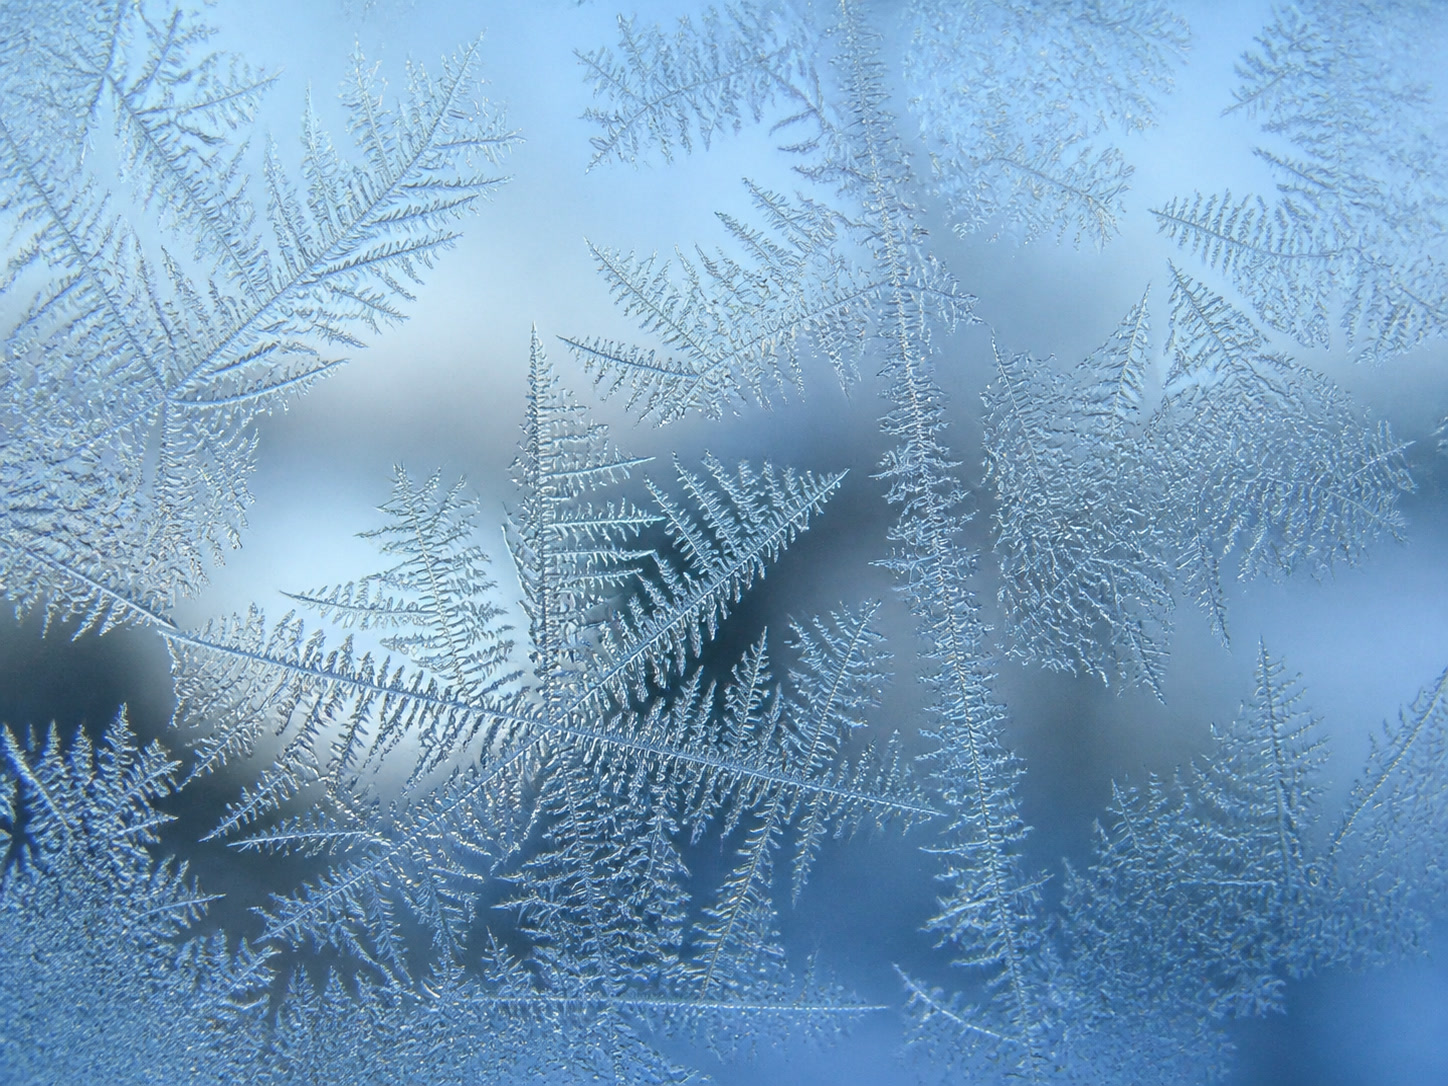
\includegraphics[width=0.5\linewidth]{images/book1/ai/g6-water-frost-window.jpg}

{\small Plumas de escarcha en un cristal helado: el agua del \omterm{def:g2:air-around-us:air}{aire} construyó este hielo durante la noche, directamente sobre el vidrio.}
\end{omfigure}

\section{Ejercicios}

\begin{exercise}[$\star$]\label{exo:g6:water-states:1}
Nombra las seis puertas de la \cref{def:g6:water-states:changes},
cada una con un avistamiento de la vida diaria.
\end{exercise}

\begin{exercise}[$\star$]\label{exo:g6:water-states:2}
¿Qué puerta: el rocío que se forma en la hierba fría al \omterm{def:g1:day-and-night:daynight}{amanecer}; \ un
muñeco de nieve que encoge un día soleado de \qty{-5}{\celsius}, sin
que aparezca ningún charco; \ unos cubitos que llenan el congelador de
``humo''?
\end{exercise}

\begin{exercise}[$\star$]\label{exo:g6:water-states:3}
Una botella cerrada de agua pesa \qty{412}{g}. \omterm{def:g2:ice-water-steam:meltfreeze}{Se congela} del todo
durante la noche. ¿Cuánto pesa ahora y qué proposición responde?
\end{exercise}

\begin{exercise}[$\star$]\label{exo:g6:water-states:4}
En el \cref{met:g6:water-states:weigh}, ¿por qué tiene que estar
tapada la botella --- y por qué hay que secarla antes de cada pesada?
\end{exercise}

\begin{exercise}[$\star$]\label{exo:g6:water-states:5}
Una olla de agua hierve destapada durante diez minutos y su
\omterm{def:g3:measuring-mass:mass}{masa} baja \qty{200}{g}. ¿Se ha destruido \omterm{def:g3:measuring-mass:mass}{masa}? ¿Dónde están esos
\omterm{def:g3:measuring-mass:units}{gramos}?
\end{exercise}

\begin{exercise}[$\star$]\label{exo:g6:water-states:6}
Un \omterm{def:g6:mass-and-volume:volume}{litro} de agua entra en el congelador. ¿Qué \omterm{def:g6:mass-and-volume:volume}{volumen} de hielo
sale, aproximadamente? La misma pregunta para la \omterm{def:g3:measuring-mass:mass}{masa}.
\end{exercise}

\begin{exercise}[$\star$]\label{exo:g6:water-states:7}
¿Por qué revientan las tuberías del agua en los inviernos duros --- y
por qué vacían los jardineros sus grifos de exterior en otoño?
\end{exercise}

\begin{exercise}[$\star$]\label{exo:g6:water-states:8}
¿Por qué \omterm{def:g1:floating-and-sinking:words}{flota} el hielo en el agua? Conecta la
\cref{prop:g6:water-states:volume} con la regla de la flotación ---
¿más ligero o más pesado a igualdad de sitio?
\end{exercise}

\begin{exercise}[$\star\star$]\label{exo:g6:water-states:9}
Cuenta el ciclo del agua como un libro de cuentas: sigue \qty{1}{kg}
de agua de mar por el bucle completo, nombrando cada puerta por la que
pasa y diciendo su \omterm{def:g3:measuring-mass:mass}{masa} en cada etapa.
\end{exercise}

\begin{exercise}[$\star\star$]\label{exo:g6:water-states:10}
Un vaso de limonada está lleno hasta el borde mismo, con cubitos
bailando. Un invitado teme que se desborde cuando el hielo
se derrita. Usa las dos auditorías (la \omterm{def:g3:measuring-mass:mass}{masa} conservada y el
sitio extra del hielo devuelto) para tranquilizar --- o alarmar --- al
invitado, con tu razonamiento.
\end{exercise}

\begin{exercise}[$\star\star$]\label{exo:g6:water-states:11}
Aparecen plumas de escarcha en un cristal helado durante la noche, en
una habitación seca, sin lluvia y con el cristal seco a la hora de
acostarse. ¿Qué puerta tomó el agua, desde dónde y por qué esa puerta
no se llama ``congelación''?
\end{exercise}

\begin{exercise}[$\star\star\star$]\label{exo:g6:water-states:12}
Los estanques se congelan de arriba abajo. Explica la cadena
entera: por qué el hielo del agua más fría se forma \emph{en la
superficie} y se queda ahí, qué le hace esa tapa flotante al flujo de
\omterm{def:g5:heat-and-insulation:heat}{calor} de debajo (una idea de aislamiento del año pasado) y por qué
los peces del fondo les deben sus inviernos al extraño hinchamiento
del agua.
\end{exercise}

\section{Problema: un kilogramo alrededor del mundo}

\begin{problem}[{Problema de fin de semana --- un kilogramo de agua
de mar en su gran gira; seis puertas, tres montañas, un libro de
cuentas sin cuadrar nunca mal}]\label{pb:g6:water-states:1}
Ponemos una etiqueta imaginaria a \qty{1}{kg} de agua de mar y lo
seguimos durante un año.

\medskip\noindent\textbf{Parte I --- Hacia arriba.}
\begin{enumerate}
  \item Junio: el Sol calienta la superficie del mar y nuestro
        \omterm{def:g3:measuring-mass:units}{kilogramo} sube al \omterm{def:g2:air-around-us:air}{aire}, invisible. Nombra la puerta que
        tomó.
  \item ¿Cuál es la \omterm{def:g3:measuring-mass:mass}{masa} de nuestro (ya invisible) \omterm{def:g3:measuring-mass:units}{kilogramo} de
        agua? ¿Qué proposición lo garantiza?
  \item A \qty{3000}{m}, el \omterm{def:g2:air-around-us:air}{aire} está frío: el agua se convierte en
        una nube de gotitas. Nombra esta puerta.
  \item Con más frío todavía, las gotitas se convierten en copos de
        nieve. Nombra esa puerta --- la \omterm{def:g6:water-states:changes}{solidificación} --- y di a
        qué \omterm{def:g3:temperature-thermometers:temperature}{temperatura} empiezan a \omterm{def:g2:ice-water-steam:meltfreeze}{congelarse} las gotitas de
        nube de agua pura.
\end{enumerate}

\medskip\noindent\textbf{Parte II --- Las cuentas del glaciar.}
Nuestro \omterm{def:g3:measuring-mass:units}{kilogramo} aterriza en un glaciar y se prensa hasta
convertirse en hielo de glaciar.
\begin{enumerate}[resume]
  \item Como agua, nuestro \omterm{def:g3:measuring-mass:units}{kilogramo} ocupaba \qty{1}{L}. ¿Qué
        \omterm{def:g6:mass-and-volume:volume}{volumen} ocupa aproximadamente como hielo?
  \item El frente del glaciar \omterm{def:g2:ice-water-steam:meltfreeze}{se derrite} en verano. Nuestro
        \omterm{def:g3:measuring-mass:units}{kilogramo} se convierte en agua de deshielo: ¿cuál es ahora su
        \omterm{def:g3:measuring-mass:mass}{masa} y cuál su \omterm{def:g6:mass-and-volume:volume}{volumen} (otra vez como agua
        líquida)?
  \item Bajando la montaña, \qty{250}{g} de nuestro \omterm{def:g3:measuring-mass:units}{kilogramo}
        se evaporan en la poza soleada de una cascada. ¿Cuánta agua
        etiquetada sigue como \omterm{def:g3:solids-liquids-gases:liquid}{líquido} en el arroyo?
  \item ¿Ha salido de la auditoría el cuarto evaporado? Di dónde
        están sus \qty{250}{g} y qué puerta tomarán con mayor
        probabilidad a continuación.
\end{enumerate}

\medskip\noindent\textbf{Parte III --- A casa y con las cuentas
cuadradas.}
\begin{enumerate}[resume]
  \item Los \qty{750}{g} del arroyo llegan al mar en octubre. Los
        \qty{250}{g} evaporados cayeron como lluvia sobre la costa en
        agosto y corrieron hasta el mar en septiembre. Suma lo que el
        mar recuperó de nuestro \omterm{def:g3:measuring-mass:units}{kilogramo}.
  \item A lo largo de toda la gira, nuestro \omterm{def:g3:measuring-mass:units}{kilogramo} no estuvo sin
        \omterm{def:g4:weight-and-mass:weight}{peso} ni un instante --- pero estuvo \emph{invisible} dos
        veces. ¿En qué etapas y en qué estado?
  \item Un compañero de clase objeta: ``La nieve es esponjosa y
        ligera --- seguro que el \omterm{def:g3:measuring-mass:units}{kilogramo} pesaba menos hecho
        nieve''. Deshaz el enredo con la pareja de palabras correcta
        de este año.
  \item Escribe la gira como una cadena de puertas, en orden, usando
        únicamente los seis nombres formales de la
        \cref{def:g6:water-states:changes}.
\end{enumerate}
\end{problem}
